\documentclass{article}
\usepackage{amsmath}

\usepackage{xcolor}
\usepackage{listings}
\usepackage{microtype}
\usepackage{graphicx}
\usepackage{float}
\lstset{
    breaklines=true,
    breakatwhitespace=true, % Bricht nur an Leerzeichen um, nicht mitten im Wort
    basicstyle=\ttfamily\small
}

\lstdefinelanguage{Rust}{
    % Core keywords
    keywords={fn, let, mut, match, return, if, else, for, while, loop, impl, struct, enum, pub, use, trait, type, crate, mod, as, break, continue, move, ref, where},
    keywordstyle=\color{blue}\bfseries,
    % Standard library types and built-ins
    ndkeywords={bool, u8, u16, u32, u64, f32, f64, i8, i16, i32, i64, usize, isize, String, Vec, Option, Result, Self},
    ndkeywordstyle=\color{purple}\bfseries,
    sensitive=true,
    comment=[l]{//},
    morecomment=[s]{/*}{*/},
    commentstyle=\color{gray}\ttfamily,
    stringstyle=\color{red}\ttfamily,
    morestring=[b]",
    morestring=[b]'
}

\begin{document}

    \section{Physikalischer Kern: Strahlensegmentschnitt}
    \label{sec:ray_intersection}

    \subsection{Visualisierung und diagnostisches Tooling}
    \label{subsec:visualizer}

    Da die Berechnung von Millionen stochastischer Strahlengänge in einem rein textbasierten oder binären Output nur schwer auf algorithmische Korrektheit überprüfbar ist,
    wurde eine Pipeline für dediziertes visuelles Debugging entwickelt (\texttt{export\_visualisation\_data}).
    Hierfür exportiert die Rust-Engine eine repräsentative Teilmenge der berechneten Strahlensegmente (\texttt{rays}),
    die Position der Schallquelle (\texttt{speaker}) sowie die Mikrofonkoordinaten samt Radius (\texttt{mic}, \texttt{mic\_radius}) in eine strukturierte JSON-Datei (\texttt{visualisation\_data.json}).

    \paragraph{Phase 1: Statische 2D-Visualisierung}
    In der initialen Entwicklungsphase der 2D-Engine wurde ein Python-Skript basierend auf der Bibliothek \texttt{matplotlib} eingesetzt.
    Dieses Werkzeug parste die geometrischen Daten und stellte sie in einem kartesischen 2D-Koordinatensystem grafisch dar.
    Dieses statische Debugging-Werkzeug war ausreichend und maßgeblich für die Identifikation tiefliegender mathematischer Anomalien in der Ebene, wie beispielsweise dem Fließkomma-Fehler bei der Reflexion (siehe Abschnitt~\ref{subsec:epsilon_fix}).

    \paragraph{Phase 2: Interaktive 3D-Volumenvisualisierung}
    Mit der Erweiterung der Simulationsarchitektur auf eine vollständige dreidimensionale Raumgeometrie stieß eine planare Projektion an ihre analytischen Grenzen.
    Komplexe räumliche Reflexionsmuster ließen sich in 2D nicht mehr nachvollziehen.
    Daher wurde das Tooling um einen interaktiven 3D-Visualizer auf Basis der Bibliothek \texttt{plotly} erweitert.

    Dieses Diagnosewerkzeug generiert einen dreidimensionalen Raum, in dem die Mikrofonkapsel nicht mehr als flacher Kreis, sondern als volumetrisches Kugel-Mesh (\texttt{go.Surface}) gerendert wird.
    Um bei der Verfolgung multipler Reflexionen die visuelle Unterscheidbarkeit einzelner Strahlengänge zu gewährleisten,
    implementiert das Skript eine farbliche Differenzierung auf Basis des Goldenen Winkels ($137{,}5^\circ$Farbton-Verschiebung im HSL-Farbraum).

    \begin{lstlisting}[language=Python]
        Python
        {ray_colour = f'hsl({(i*137.5)%360},80%,60%)'}
    \end{lstlisting}
    Die interaktive Natur der \texttt{plotly}-Bibliothek erlaubt es, die Raumgeometrie zur Laufzeit zu rotieren und zu zoomen.
    \begin{figure}[H]
        \centering % Zentriert das Bild auf der Seite

        % 3. Das eigentliche Bild einfügen und skalieren
        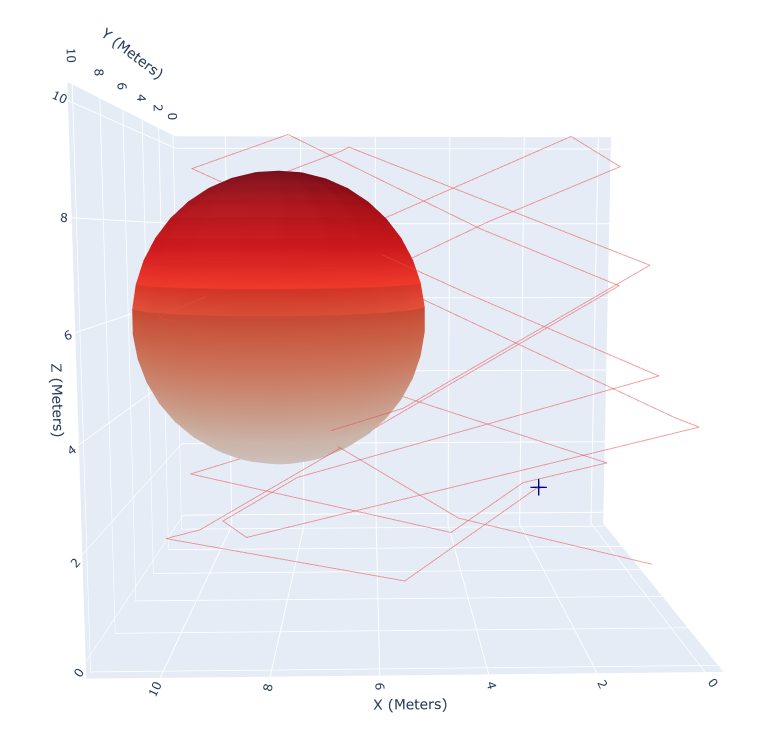
\includegraphics[width=0.8\textwidth]{3dplot3}

        \caption{Ein Strahl, rote Sphäre = Mikrofonradius, Blaues kreuz = Lautsprecher} % Bildunterschrift
        \label{fig:3dplot3} % Textmarke für Querverweise
    \end{figure}
    Dies war unerlässlich, um räumliche Anomalien und fehlerhafte Vektorreflexionen im 3D-Raum zu identifizieren.

    \subsection{Behandlung von Fließkomma-Ungenauigkeiten (Self-Intersection)}
    \label{subsec:epsilon_fix}

    Die erste Auswertung der Strahlengänge durch den Visualizer offenbarte ein kritisches algorithmisches Problem:
    Strahlen wurden unregelmäßig terminiert oder verblieben an Wänden, ohne weiter zu reflektieren.
    Die Ursache hierfür lag in der Fließkomma-Ungenauigkeit der CPU.

    Wenn ein Strahlengang an einer Wand reflektiert wird (z.\,B. bei exakt $t=5{,}0$),
    dient dieser mathematische Schnittpunkt als Ursprung für den nachfolgenden Reflexionsstrahl.
    In der darauffolgenden Iteration prüft die Engine diesen neuen Strahl gegen alle Wände des Raumes inklusive der Wand, auf der er sich bereits befindet.
    Aufgrund mikroskopischer Rundungsfehler berechnet der Schnittpunktalgorithmus die Distanz zur aktuellen Wand nicht als exakt $0{,}0$, sondern beispielsweise als $-0{,}0000001$.
    \begin{figure}[H]
        \centering % Zentriert das Bild auf der Seite

        % 3. Das eigentliche Bild einfügen und skalieren
        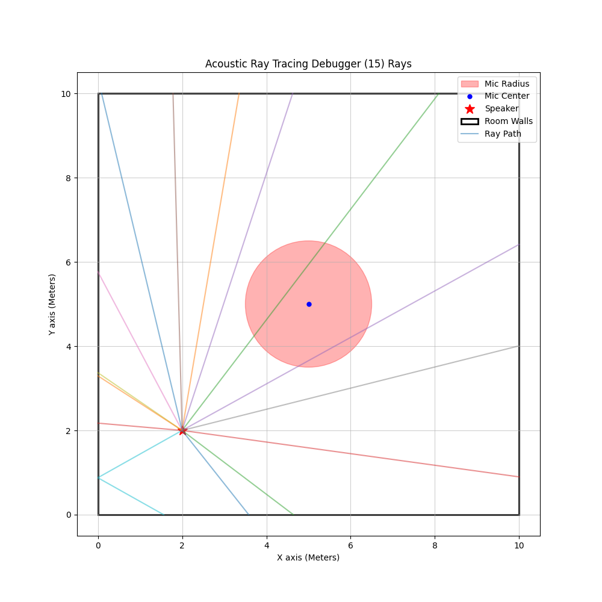
\includegraphics[width=1.0\textwidth]{shadowacne1}

        \caption{2D-Visualizer, Türkiser Strahl hier -0,000002 beim ersten bounce} % Bildunterschrift
        \label{fig:shadowacne1} % Textmarke für Querverweise
    \end{figure}

    Die ursprüngliche Abbruchbedingung der Engine lautete:
    \[ \text{if ray\_t} < 0.0 \{ \text{return None;} \} \]
    Da Werte wie $0{,}0000000$ (oder mikroskopisch positive Werte) nicht strikt kleiner als $0{,}0$ sind, registrierte die Engine fälschlicherweise einen sofortigen, validen Treffer auf derselben Wand.
    Der Strahl ,,reflektierte`` in einer Endlosschleife mit der Distanz $0{,}0$ am selben Punkt, bis das konfigurierte Limit maximaler Reflexionen (\texttt{max\_bounces})
    in Bruchteilen einer Millisekunde erschöpft war.
    Daraufhin wurde der Strahl fälschlicherweise terminiert.
    In der Computergrafik ist dieses Phänomen auch als \emph{Shadow Acne} oder \emph{Self-Intersection} bekannt.


    Zur Lösung dieses Problems wurde ein Epsilon-Wert ($\epsilon$) eingeführt.
    Die Bedingung wurde zu \texttt{if ray\_t < 0.001 \{ return None; \}} modifiziert.
    Ein berechneter Schnittpunkt wird folglich nur dann als valide betrachtet,
    wenn der Strahl eine physikalische Mindestdistanz von $1\,\text{mm}$ zurückgelegt hat.
    Die erneute Visualisierung bestätigte, dass die Strahlen die Oberflächen nun korrekt verließen und
    das physikalische Reflexionsverhalten korrekt simuliert wurde.
    \begin{figure}[htbp]
        \centering % Zentriert das Bild auf der Seite

        % 3. Das eigentliche Bild einfügen und skalieren
        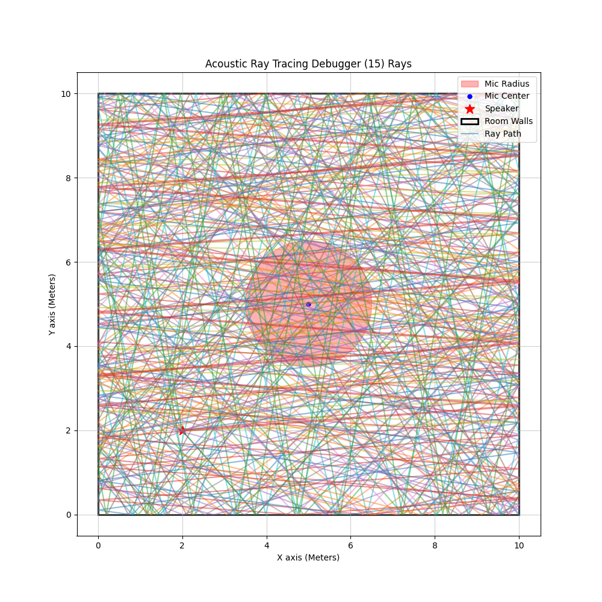
\includegraphics[width=1.0\textwidth]{fixedshadowacne}

        \caption{2D-Visualizer, mit Epsilon wert} % Bildunterschrift
        \label{fig:shadowacne2} % Textmarke für Querverweise
    \end{figure}


\end{document}